\documentclass[12pt,pdf,aspectratio=169,t]{beamer}

\usefonttheme[onlymath]{serif}
\usepackage{amsmath,amsfonts,amssymb,amsthm,mathtools}
\usepackage[T2A]{fontenc}
\usepackage[utf8]{inputenc}
\usepackage[english]{babel}
\usepackage{ragged2e}
\usepackage{indentfirst}
\usepackage{dsfont}
\justifying
\setlength{\parindent}{1em}
\setbeamertemplate{navigation symbols}{}
\addtobeamertemplate{frametitle}{\setlength{\parindent}{0em}}{}
\addtobeamertemplate{navigation symbols}{}{%
    \usebeamerfont{footline}%
    \usebeamercolor[fg]{footline}%
    \hspace{1em}%
    \insertframenumber/\inserttotalframenumber
}
\setbeamertemplate{frametitle continuation}{}
\allowdisplaybreaks[1]
\mathtoolsset{showonlyrefs}
\usepackage{graphicx}
\usepackage{vcell}

\usepackage{tikz}
\usepackage{pgfplots}
\pgfplotsset{compat=1.17}
\usetikzlibrary{positioning,arrows.meta,shapes}


\renewcommand{\P}[1]{\mathbb{P}\left(#1\right)}

\newcommand{\Pn}[1]{\mathbb{P}'\left(#1\right)}
\newcommand{\E}{\mathbb{E}}
\newcommand{\D}{\mathbb{D}}
\newcommand{\N}{\mathbb{N}}
\newcommand{\Z}{\mathbb{Z}}
\newcommand{\R}{\mathbb{R}}
\newcommand{\X}{\mathbb{X}}
\newcommand{\g}{\gamma}
\newcommand{\Poiss}[1]{\mathrm{Pois}\left(#1\right)}
\newcommand{\Unif}[1]{\mathrm{U}\left(#1\right)}
\newcommand{\Exp}[1]{\mathrm{Exp}\left(#1\right)}
\newcommand{\Sym}[1]{\mathrm{S}_{#1}}
\newcommand{\ESF}[1]{\mathrm{ESF}\left(#1\right)}
\DeclareMathOperator{\card}{card}
\DeclarePairedDelimiter\ceil{\lceil}{\rceil}
\DeclarePairedDelimiter\floor{\lfloor}{\rfloor}
\DeclareMathOperator{\Sum}{sum}
\renewcommand{\L}[1]{\mathcal{L}\left\{#1\right\}}
\DeclareMathOperator{\smax}{s-max}
\DeclareMathOperator{\smin}{s-min}
\DeclareMathOperator{\cycle}{c}
\DeclareMathOperator{\inv}{i}
\newcommand{\cov}[2]{\mathrm{cov}\left(#1, #2\right)}

\renewcommand{\d}{\mathrm{d}}

\newcommand*{\defeq}{\stackrel{\text{def}}{=}}
\makeatletter
\newcommand\incircbin
{%
  \mathpalette\@incircbin
}
\newcommand\@incircbin[2]
{%
  \mathbin%
  {%
    \ooalign{\hidewidth$#1#2$\hidewidth\crcr$#1\bigcirc$}%
  }%
}
\newcommand{\oeq}{\incircbin{=}}
\makeatother

\newtheorem{theorem}{Теорема}[section]
\newtheorem*{theorem*}{Теорема}
\newtheorem{corollary}{Наслідок}[theorem]
\newtheorem{lemma}[theorem]{Лема}
\newtheorem*{remark}{Зауваження}

\theoremstyle{definition} % "Определение"
\newtheorem{definition}{Означення}[section]
\newtheorem*{definition*}{Означення}

\usetheme{Luebeck}
\title{Limit theorems for fixed points \linebreak of Ewens random permutations}
\author[Oleksii Galganov]{Oleksii Galganov\\{\fontsize{9pt}{11pt}\selectfont based on recent joint work \\ \vspace{-0.5em} with Andrii Ilienko}}
\institute{
    National Technical University of Ukraine \\
    «Igor Sikorsky Kyiv Polytechnic Institute», \\
    Institute for Applied System Analysis, \\
    Ukraine, Kyiv
}

\date{The Skorokhod readings, 7 June 2022}
\begin{document}
    \begin{frame}
        \titlepage
    \end{frame}
    \begin{frame}
        \frametitle{Outline}
        \begin{enumerate}
            \item Ewens permutations
            \item Vague convergence to Poisson process
            \item Limit theorems for statistics
            \item Modelling methods overview
            \item Perspectives
        \end{enumerate}
    \end{frame}
    \begin{frame}
        \frametitle{Ewens permutations}
        Consider the following probability measure on
        symmetric group $\Sym{n}$:
        \begin{equation}\label{ESF}
            \mathbb{P}(\{\pi\}) = \frac{
                \theta^{\cycle(\pi)}
            }{
                \theta_{(n)}
            }, \; \pi \in \Sym{n},
        \end{equation}
        where $\theta > 0$ is a fixed parameter, $\cycle(\pi)$ denotes the number of cycles in $\pi$
        and $\theta_{(n)} = \theta (\theta + 1) \dots (\theta + n - 1)$.
        
        \eqref{ESF} is known as the \emph{Ewens distribution}
        on $\Sym{n}$. For $\theta = 1$, it reduces to the uniform distribution,
        which assigns probability $\frac{1}{n!}$ to each $\pi \in \Sym{n}$.
    \end{frame}
    \begin{frame}
        \frametitle{Ewens permutations}
        Let $\sigma$ be distributed as \eqref{ESF}, and $\cycle_j(\sigma)$ stands for
        the number of cycles of length $j$ in $\sigma$.
        For $c_1, ..., c_n \in \N_0$ with $\sum_{j=1}^n j c_j = n$ 
        formula \eqref{ESF} results in
        \begin{gather}\label{ESF_original}
            \P{\cycle_1(\sigma) = c_1,...,\cycle_n(\sigma) = c_n} =
            \frac{n!}{\theta_{(n)}} 
            \prod_{j=1}^n \left(\frac{\theta}{j}\right)^{c_j} \frac{1}{c_j!}.
        \end{gather}

        \eqref{ESF_original} is known as the celebrated
        \emph{Ewens sampling formula} (Ewens, 1972) which originally
        came from population genetics and subsequently found
        numerous applications in combinatorial stochastic
        processes, Bayesian nonparametrics, inductive inference, etc. (Crane, 2016)
    \end{frame}
    \begin{frame}
        \frametitle{Ewens permutations}
        As is customary in the literature, we will in what follows denote
        the Ewens distribution \eqref{ESF} by $\ESF{n, \theta}$ and write
        $\sigma \sim \ESF{n, \theta}$.

        There is a classic result (Arratia, Barbour, Tavaré, 1992)
        about limiting distribution of cycle counts for Ewens permutation:
        \begin{gather}\label{ABT_convergence}
            \left(\cycle_1(\sigma_n), \cycle_2(\sigma_n), \cycle_3(\sigma_n), ...\right)
            \overset{d}{\longrightarrow}
            \left(X_1, X_2, X_3, ...\right), \; n\to\infty,
        \end{gather}
        where $\left(X_j, j \geq 1\right)$ are independent
        $\Poiss{\theta / j}$ random variables.

        We will focus on the limiting behavior of fixed points, the total
        number of which is, accordingly to \eqref{ABT_convergence},
        asymptotically $\Poiss{\theta}$.
    \end{frame}
    \begin{frame}
        \frametitle{Vague convergence to Poisson process}
        Let's define a sequence of point processes $\left(P_n, n \geq 1\right)$ on $[0, 1]$
        by
        \begin{gather}\label{Pn_def}
            P_n = \sum_{i=1}^n \delta_{\frac{i}{n}} \mathds{1} \left\{\sigma_n(i) = i\right\},
        \end{gather}
        where $\sigma_n \sim \ESF{n, \theta}$, and $\delta_x$ denotes Dirac measure at $x$.

        Specifically, $P_n([0, 1]) = c_1(\sigma_n)$ is the number of fixed points of $\sigma_n$.
        
        In which sense can $P_n$ converge and what can limit be equal to?
    \end{frame}
    \begin{frame}
        \frametitle{Vague convergence to Poisson process}
        \begin{definition}[vague topology]
            Let $\left(\mu_n, n \geq 1\right)$ be a sequence of
            measures on a metric space $E$. This sequence 
            \emph{converges vaguely} to the measure $\xi$ if
            $\int_E f \d \mu_n \to \int_E f \d \mu$ for each
            non-negative continuous compactly supported test function $f$.
        \end{definition}
        \begin{definition}[vague convergence in distribution]
            Let $\left(\xi_n, n\geq 1\right)$ be a sequence of
            point processes on a metric space $E$. This sequence
            \emph{vaguely converges in distribution} to the point process $\xi$ if
            $\E\varphi(\xi_n) \to \E\varphi(\xi)$ for each
            bounded and continuous w.r.t. vague topology
            $\varphi: M_p(E) \to \R$, 
            which is denoted by 
            $\xi_n \overset{vd}{\longrightarrow} \xi$.
        \end{definition}
    \end{frame}
    \begin{frame}
        \frametitle{Vague convergence to Poisson process}
        In case of $E = [0, 1]$, vague convergence in distribution
        is closely related to the distributional convergence of
        cumulative processes in the Skorokhod $J_1$-topology (see, e.g., Kallenberg, 2017).
        \begin{theorem}
            Let $\left(\xi_n, n\geq 1\right)$ be a sequence of
            point processes on $[0, 1]$. Then
            $\left(
                \xi_n([0, {\cdot\,}]) \overset{J_1, d}{\longrightarrow} \xi([0, {\cdot\,}])
            \right) \Rightarrow
            \left(
                \xi_n \overset{vd}{\longrightarrow} \xi
            \right)$ and two statement are equivalent, if 
            $\xi(\{0\}) = 0 \; a.s.$ and 
            $\xi$ is simple, i.e.
            $\P{\forall \; x \in [0, 1]: \xi(\{x\}) \leq 1} = 1$.
        \end{theorem}
    \end{frame}
    \begin{frame}
        \frametitle{Vague convergence to Poisson process}
        Since the limit in our core result is the homogeneous
        Poisson point process, we first recall the corresponding definition.
        \begin{definition}
            Let $\lambda > 0$, and $\mathcal{E}$ and $\mathrm{Leb}$ denote 
            the Borel sigma-algebra on $E \subset \R^d$ and
            the Lebesgue measure on $E$, respectively.
            The \emph{homogeneous Poisson point process with rate $\lambda$} is
            a point process $N$ defined by
            \begin{enumerate}
                \item For all $F \in \mathcal{E}$,
                $N(F) \sim \Poiss{\lambda \cdot \mathrm{Leb}(F)}$ if 
                $\mathrm{Leb}(F) < \infty$ and $N(F) = \infty \; a.s.$ otherwise.
                \item $\left(N(F_i), 1\leq i \leq k\right)$ are independent 
                for mutually disjoint sets $F_1, ..., F_k \in \mathcal{E}$.
            \end{enumerate}
        \end{definition}
    \end{frame}
    \begin{frame}
        \frametitle{Vague convergence to Poisson process}
        \begin{theorem}[convergence of $P_n$]
            The sequence of point processes
            $\left(P_n, n \geq 1\right)$ defined by \eqref{Pn_def}
            vaguely converges in distribution to the
            homogeneous Poisson point process $N$ with rate $\theta$:
            $P_n \overset{vd}{\longrightarrow} N$.

        \end{theorem}
        As $N$ satisfies all equivalence conditions of the preceding theorem,
        then also $P_n \overset{J_1,d}{\longrightarrow} N$ holds.

        It follows from the well-known property of 
        the homogeneous Poisson process that, 
        as $n \to \infty$, unordered (normalized by $n$) 
        positions of fixed points 
        become \emph{asymptotically independent}
        and uniformly distributed conditionally 
        on their total number. 
    \end{frame}
    \begin{frame}
        \frametitle{Vague convergence to Poisson process}
        Before we briefly describe the idea of the proof, let's take a look at
        a $vd$-convergence criterion. (Kallenberg, 2017)
        \begin{theorem}
            Let $\left(\xi_n, n\geq 1\right)$ and $\xi$ be point processes
            on a metric space $E$ with Borel sigma-algebra $\mathcal{E}$, where $\xi$ is simple, and fix a dissecting ring
            $\mathcal{U} \subset \hat{\mathcal{E}}_{\xi}$,
            where 
            $\hat{\mathcal{E}}_{\xi} = \left\{B \in \mathcal{E} : \xi(\partial B) = 0 \;a.s.\right\}$,
            and a dissecting semi-ring $\mathcal{I} \subset \mathcal{U}$.
            Then $\xi_n \overset{vd}{\longrightarrow} \xi$ iff
            \begin{enumerate}
                \item $\underset{n\to\infty}{\lim}\;\P{\xi_n(U) = 0} = \P{\xi(U) = 0}$ for $U\in\mathcal{U}$;
        \item $\underset{n\to\infty}{\limsup}\; \P{\xi_n(I) > 1} \leq \P{\xi(I) > 1}$ for $I \in \mathcal{I}$.
            \end{enumerate}
        \end{theorem}
        For our case, $\mathcal{U} = \mathcal{I}$ to be a family of
        disjoint unions of $\left<\alpha, \beta\right> \subset [0, 1]$
        will be enough, $\left<\right.$ being either $($ or $[$.
    \end{frame}
    \begin{frame}
        \frametitle{Vague convergence to Poisson process}
        The proof is based on establishing an explicit formula
        for $\P{P_n(I) = k}$, where $I = \bigvee_{j=0}^m \left<\alpha_j, \beta_j\right> \subset [0, 1]$ and
        showing that $\P{P_n(I) = k} \to \P{N(I) = k}$.

        For the sake of simplicity, we restrict ourselves here only to the case
        $I = [0, \gamma]$.
        A combinatorial argument based on the inclusion-exclusion principle leads to
        \vspace{-1em}
        \begin{gather*}
            \P{P_n([0, \gamma]) = k} = C_{\ceil*{\gamma n}}^k \sum_{i=0}^{\ceil*{\gamma n}-k} (-1)^i C_{\ceil*{\gamma n}-k}^i
            \frac{\theta^{i+k} \theta_{(n-k-i)}}{\theta_{(n)}} = \\ =
            \frac{\theta^k}{k!} \sum_{i=0}^{\ceil*{\gamma n}-k} (-1)^i \frac{\theta^i}{i!} 
            \frac{(\ceil*{\gamma n})! \cdot \theta_{(n-k-i)}}{(\ceil*{\gamma n} - k - i)! \cdot \theta_{(n)}}.
        \end{gather*}

        Then, after routine calculations and careful asymptotic analysis
        we come to $\P{P_n(I) = k} \to \frac{(\gamma \theta)^k}{k!} e^{-\gamma \theta} = \P{N(I) = k}$.
        Since both conditions for Kallenberg's $vd$-convergence criterion are fulfilled,
        it proves that $P_n \overset{vd}{\longrightarrow} N$ as $n \to \infty$.     
    \end{frame}
    \begin{frame}
        \frametitle{Limit theorems for statistics}
        Even though $P_n \overset{vd}{\longrightarrow} N$ itself
        is an interesting result, it becomes even more fruitful 
        if we consider the continuous mapping theorem.

        In our case, it can shortly be formulated as following:
        \begin{theorem}
            If $\xi_n \overset{vd}{\longrightarrow} \xi$ and
            $\varphi : M_p([0, 1]) \to \R$ s.t.
            $\xi \in C_{\varphi} \; a.s.$, then
            $\varphi(\xi_n) \overset{d}{\longrightarrow} \varphi(\xi)$.
        \end{theorem}
        Thus, we can obtain a limit theorem for any statistics of fixed points,
        provided that it can be represented as a continuous function w.r.t vague topology.

        It's worth recalling a property of $N$:
        positions of its points are uniform and independent conditioned on their number.
        In what follows, we will refer to this property as \emph{CUI}.
    \end{frame}
    \begin{frame}
        \frametitle{Limit theorems for statistics: min and max fixed points}
        \begin{theorem}
            Let $m_n$ and $M_n$ denote the smallest and the largest fixed points of $\sigma_n \sim \ESF{n, \theta}$,
            respectively, with $m_n = n+1$ and $M_n = 0$ in case there are no fixed points at all.
            Then $\frac{m_n}{n} \overset{d}{\longrightarrow} m$ and $\frac{M_n}{n} \overset{d}{\longrightarrow} M$,
            with $m$ and $M$ having CDFs 
            \begin{gather}
                F_m(x) = \begin{cases}
                    0, & x < 0, \\
                    1 - e^{-\theta x}, & 0 \leq x < 1, \\
                    1, & x \geq 1,
                \end{cases}\;
                F_M(x) = \begin{cases}
                    0, & x < 0, \\
                    e^{\theta(x - 1)}, & 0 \leq x < 1, \\
                        1, & x \geq 1.
                \end{cases}
            \end{gather}
            Furthermore, $\frac{\E m_n}{n} \to \E m = \frac{1 - e^{-\theta}}{\theta}$
            and $\frac{\E M_n}{n} \to \E M = \frac{e^{-\theta} + \theta - 1}{\theta}$.
        \end{theorem}
        This result can be proven using CUI and explicit distributions
        of the first and last order statistics of $\Unif{0, 1}$.
    \end{frame}
    \begin{frame}[allowframebreaks]
        \frametitle{Limit theorems for statistics: min and max spacings}
        Let's consider the spacings between fixed points of $\sigma_n$.
        We also introduce the initial and final spacings by placing to virtual
        fixed points at $0$ and $n+1$.
        Recalling CUI, we can study the distribution of spacings for $\Unif{0, 1}$.

        Let $S_i^{[n+1]}, i=1,...,n+1$ denote the spacings between $n$ i.i.d. $\Unif{0, 1}$ variables,
        including those starting at $0$ and ending at $1$.
        It is known (e.g., Rényi, 1953 or Holst, 1980) that for i.i.d. $X_i \sim \Exp{1}, i = 1,..., n+1$,
        \vspace{-1em}
        \begin{gather}
            \label{distr_equal_1}
            \left(
                S_1^{[n+1]}, S_2^{[n+1]}, \dots, S_{n+1}^{[n+1]}
            \right)
            \overset{d}{=}
            \left(
                \frac{X_1}{\sum_{i=1}^{n+1} X_i},
                \frac{X_2}{\sum_{i=1}^{n+1} X_i},
                \dots,
                \frac{X_{n+1}}{\sum_{i=1}^{n+1} X_i}
            \right), \\
            \label{distr_equal_2}
            \left(
                S_{(1)}^{[n+1]}, S_{(2)}^{[n+1]}, \dots, S_{(n+1)}^{[n+1]}
            \right)
            \overset{d}{=}
            \left(
                \frac{X_{(1)}}{\sum_{i=1}^{n+1} X_i},
                \frac{X_{(2)}}{\sum_{i=1}^{n+1} X_i},
                \dots,
                \frac{X_{(n+1)}}{\sum_{i=1}^{n+1} X_i}
            \right), 
        \end{gather}
        \begin{gather}
            \label{distr_equal_3}
            X_{(i)} \overset{d}{=}
            \frac{X_{n+1}}{n+1} + \frac{X_{n}}{n} + \dots + \frac{X_{n-i+2}}{n-i+2} = 
            \sum_{k=0}^{i-1} \frac{X_{n+1-k}}{n+1-k}.
        \end{gather}
        One can also prove the following equalities:
        \begin{gather}\label{distr_equal_4}
            S_{(i)}^{[n+1]} \overset{d}{=}
            \frac{
                \frac{X_{n+1}}{n+1} + \frac{X_{n}}{n} + \dots + \frac{X_{n-i+2}}{n-i+2}
            }{
                \sum_{j=1}^{n+1} X_j
            } = \frac{
                \sum_{k=0}^{i-1} \frac{X_{n+1-k}}{n+1-k}
            }{
                \sum_{j=1}^{n+1} X_j
            }, \; i = 1, \dots, n+1.
        \end{gather}

        Together with CUI, equalities 
        $S_{(1)}^{[n+1]} \overset{d}{=} \frac{X_{n + 1}}{(n + 1)\sum_{i=1}^{n+1} X_i}$ and 
        $S_{(n+1)}^{[n+1]} = \frac{\sum_{i=1}^{n+1} \frac{X_i}{i}}{\sum_{i=1}^{n+1} X_i}$ lead to the following result:
        \pagebreak
        \begin{theorem}
            Let $\delta_n$ and $\Delta_n$ denote the smallest and the largest
            spacings between fixed points of $\sigma_n \sim \ESF{n, \theta}$, respectively.
            Then $\frac{\delta_n}{n} \overset{d}{\longrightarrow} \delta$ and 
            $\frac{\Delta_n}{n} \overset{d}{\longrightarrow} \Delta$ with
            \begin{gather}
                \delta \overset{d}{=}
                \frac{X_{\nu + 1}}{(\nu + 1)\sum_{i=1}^{\nu+1} X_i}, \;
                \Delta \overset{d}{=} 
                \frac{\sum_{i=1}^{\nu+1} \frac{X_i}{i}}{\sum_{i=1}^{\nu+1} X_i},
            \end{gather}
            where $\left(X_i, i\geq 1\right)$ are 
            independent $\Exp{1}$ variables and $\nu \sim \Poiss{\theta}$
            is independent of $\left(X_i, i\geq 1\right)$.

            Furthermore, $\frac{\E \delta_n}{n} \to \E \delta = \frac{e^{-\theta}}{\theta} \int_0^{\theta} \frac{e^t - 1}{t} \d t$
            and $\frac{\E \Delta_n}{n} \to \E \Delta = \frac{1}{\theta} \int_0^{\theta} \frac{1 - e^{-t}}{t} \d t$.
        \end{theorem}
    \end{frame}
    \begin{frame}[allowframebreaks]
        \frametitle{Limit theorems for statistics: sum of fixed points}
        \begin{theorem}
            Let $S_n$ denote the sum of the fixed points of $\sigma_n \sim \ESF{n, \theta}$.
            Then $\frac{S_n}{n} \overset{d}{\longrightarrow} S$ with 
            \vspace{-1em}
            \begin{gather}
                F_{S}(x) = e^{-\theta}
                \sum\limits_{k=0}^{\floor*{x}}
                (-1)^k \frac{1}{k!}\left(\theta(x-k)\right)^{\frac{k}{2}} I_k\left(2\sqrt{\theta(x-k)}\right),
            \end{gather}
            and Laplace transform given by
            \vspace{-1em}
            \begin{gather}
                \E e^{-p S} = \exp\left\{- \theta \left( 1 + \frac{1}{p}(e^{-p} - 1)\right) \right\}.
            \end{gather}
            \vspace{-1em}
        \end{theorem}
        Here $I_k(z) = \left(\frac{1}{2} z\right)^{k}
            \sum_{m=0}^{\infty} \frac{
                \left(\frac{1}{4} z^2 \right)^{m}
            }{
                m! (k + m)!
            } = \frac{1}{\pi} \int_0^{\pi} e^{z \cos t} \cos{(kt)} \d t$ is the modified Bessel function of the first kind.

            In order to get the explicit distribution of $S$, we use CUI with some rather involved calculus,
            and Laplace functional of $N$ (e.g., Resnick, 2008).
            The density of its (normalized) absolutely continuous component $\widehat{S}$ is 
            $f_{\widehat{S}}(x) = \frac{\theta e^{-\theta}}{1 - e^{-\theta}}
            \sum_{k=0}^{\floor*{x}} \frac{(-1)^k}{k!} f_k(x)$, where
            $$f_k(x) = \left(\theta (x - k)\right)^{\frac{k}{2} - 1}
            \left(
                k I_k \left(2 \sqrt{\theta (x - k)} \right) + 
                \sqrt{\theta (x - k)} I_{k+1} \left(2 \sqrt{\theta (x - k)}\right)
            \right).$$
            $\widehat{S}$ can be considered as the distributional limit of the sum
            of fixed points conditioned on the event that there is at least one such point.

            \begin{center}
                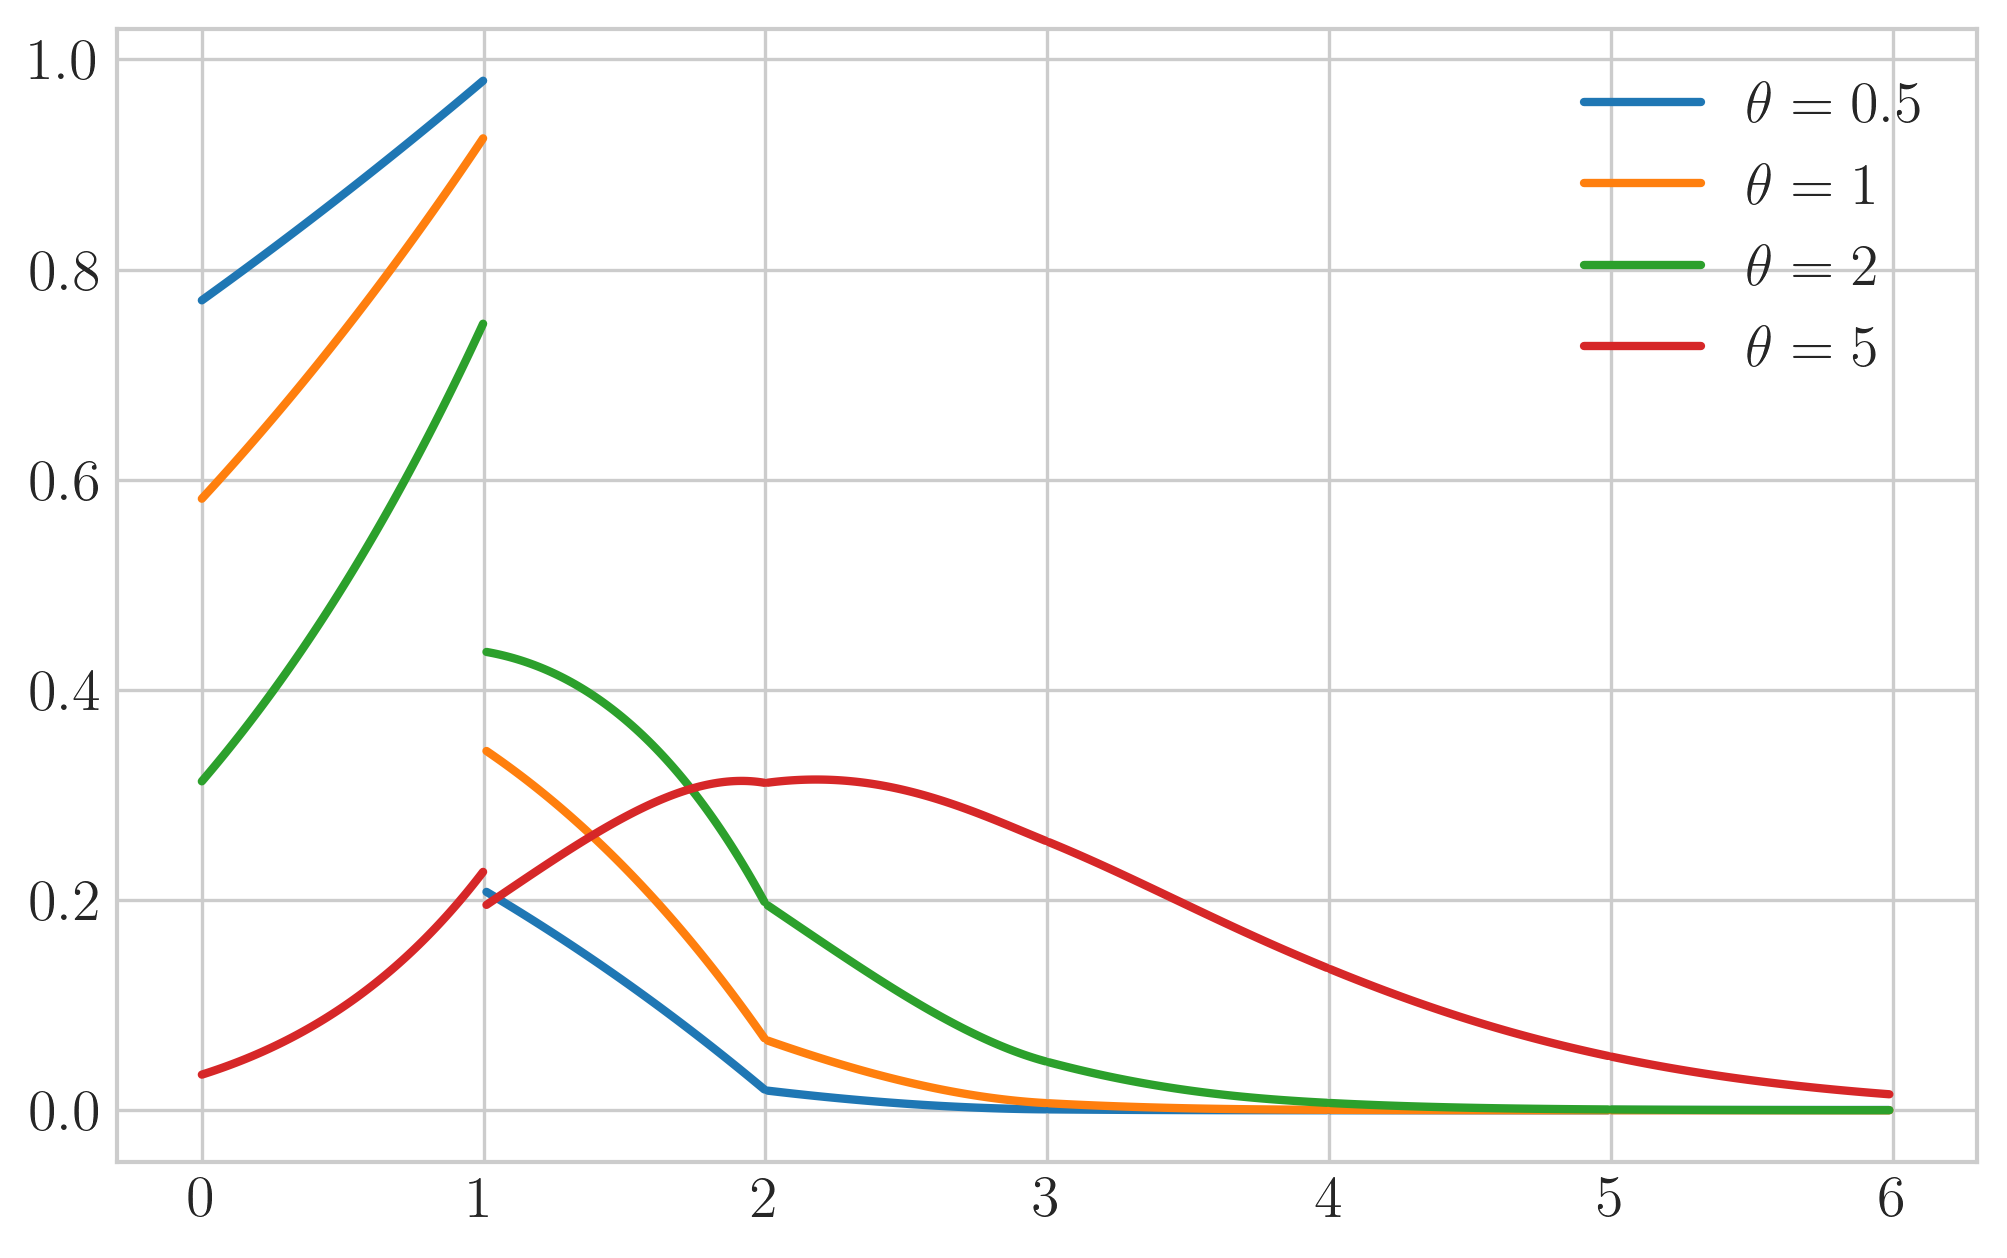
\includegraphics[scale=0.55]{plots/pdf_sum_hat.png}
    
                Plots of $f_{\widehat{S}}(x)$ for different values of $\theta$.
            \end{center}
    \end{frame}
    \begin{frame}[allowframebreaks]
        \frametitle{Modelling methods overview}
        As it is computationally inefficient to sample Ewens permutations directly from $\Sym{n}$,
        modelling can be done by means of various couplings, which can also bring some useful properties. 
        (Arratia, Barbour, Tavaré, 1992)
        \begin{enumerate}
            \item \emph{Chinese restaurant process (CRP)} is used to generate a sequence 
            $\left(\sigma_i, i\geq 1\right)$ of
            $\sigma_i \sim \ESF{i, \theta}$ on a common probability space. Let $\left(A_i, i\geq 1\right)$
            be a sequence of independent random variables defined by
            \begin{gather}
                \P{A_i = j} = \begin{cases}
                    \frac{\theta}{\theta + i - 1}, & j = i, \\
                    \frac{1}{\theta + i - 1}, & j = 1, 2, ..., i-1.
                \end{cases}
            \end{gather}
            First cycle starts with $1$. As the first $n-1$ integers have been assigned to cycles,
            $n$ starts a new cycle with probability $\P{A_n = n}$, or place to the right of $j$
            with probability $\P{A_n = j}$.
            
            \begin{center}
                \scalebox{0.7}{
                    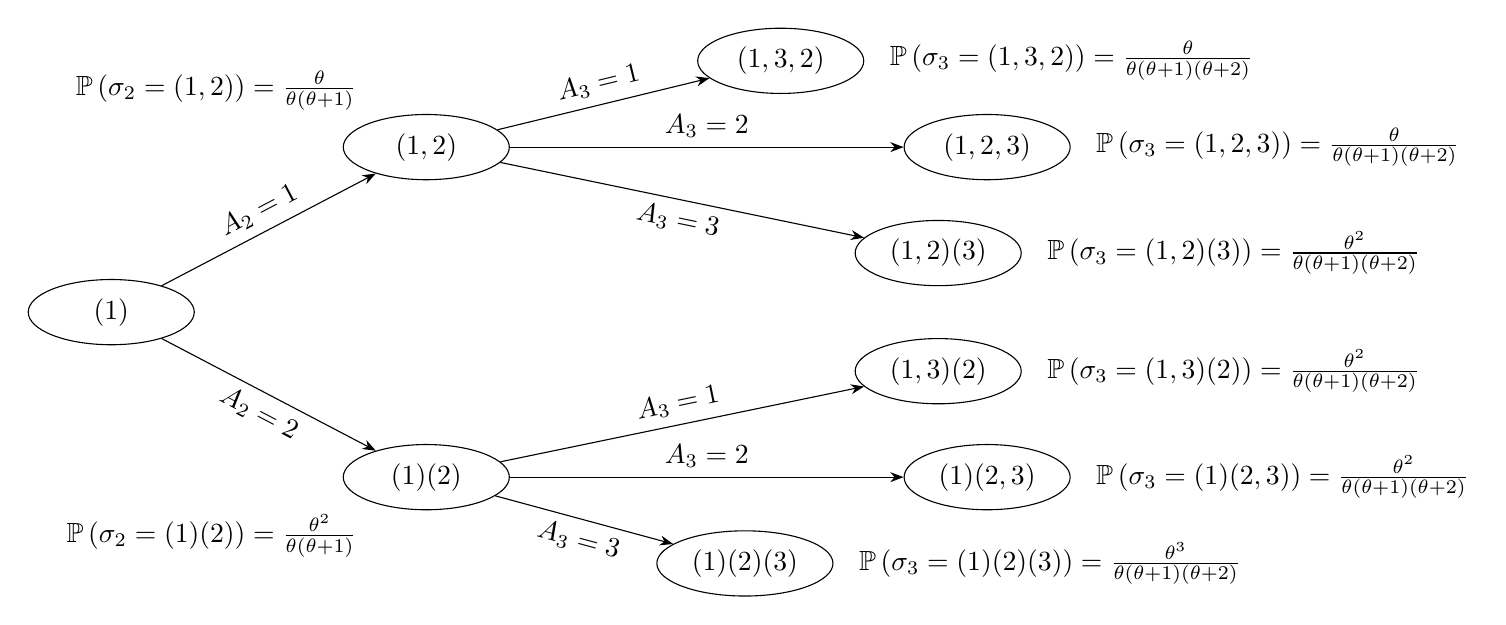
\begin{tikzpicture}[auto,vertex/.style={draw,ellipse,minimum width=60pt}]
                        \node[vertex] (one) {$(1)$};
                        \node[vertex, above right=1.5cm and 2.5cm of one] (onetwo) {$(1, 2)$};
                        \node[vertex, below right=1.5cm and 2.5cm of one] (one_two) {$(1) (2)$};
                        \node[vertex, right=5cm of onetwo] (onetwothree) {$(1, 2, 3)$};
                        \node[vertex, below right=0.75 and 5cm of onetwo] (onetwo_three) {$(1, 2) (3)$};
                        \node[vertex, above right=0.5cm and 3cm of onetwo] (onethreetwo) {$(1, 3, 2)$};
                        \node[vertex, above right=0.75cm and 5cm of one_two] (onethree_two) {$(1, 3) (2)$};
                        \node[vertex, right=5cm of one_two] (one_twothree) {$(1) (2, 3)$};
                        \node[vertex, below right=0.5cm and 2.5cm of one_two] (one_two_three) {$(1) (2) (3)$};
                        \path[-{Stealth[]}, every node/.style={sloped,anchor=south,auto=false}]
                            (one) edge node {$A_2 = 1$} (onetwo)
                            (one) edge node[below] {$A_2 = 2$} (one_two)
                            (onetwo) edge node {$A_3 = 2$} (onetwothree)
                            (onetwo) edge node {$A_3 = 1$} (onethreetwo)
                            (onetwo) edge node[below] {$A_3 = 3$} (onetwo_three)
                            (one_two) edge node {$A_3 = 1$} (onethree_two)
                            (one_two) edge node {$A_3 = 2$} (one_twothree)
                            (one_two) edge node[below] {$A_3 = 3$} (one_two_three);
                        \node[right=0.2cm of onethreetwo] {$\P{\sigma_3 = (1, 3, 2)} = \frac{\theta}{\theta (\theta + 1)(\theta + 2)}$};
                        \node[right=0.2cm of onetwothree] {$\P{\sigma_3 = (1, 2, 3)} = \frac{\theta}{\theta (\theta + 1)(\theta + 2)}$};
                        \node[right=0.2cm of onetwo_three] {$\P{\sigma_3 = (1, 2) (3)} = \frac{\theta^2}{\theta (\theta + 1)(\theta + 2)}$};
                        \node[right=0.2cm of onethree_two] {$\P{\sigma_3 = (1, 3) (2)} = \frac{\theta^2}{\theta (\theta + 1)(\theta + 2)}$};
                        \node[right=0.2cm of one_twothree] {$\P{\sigma_3 = (1) (2, 3)} = \frac{\theta^2}{\theta (\theta + 1)(\theta + 2)}$};
                        \node[right=0.2cm of one_two_three] {$\P{\sigma_3 = (1) (2) (3)} = \frac{\theta^3}{\theta (\theta + 1)(\theta + 2)}$};
                        \node[above left=0.05cm and 0.01cm of onetwo] {$\P{\sigma_2 = (1, 2)} = \frac{\theta}{\theta (\theta + 1)}$};
                        \node[below left=0.05cm and 0.01cm of one_two] {$\P{\sigma_2 = (1)(2)} = \frac{\theta^2}{\theta (\theta + 1)}$};
                    \end{tikzpicture}
                }

                An example of how CRP generates Ewens permutations for $n = 3$.
            \end{center}
            \item \emph{Feller coupling} only allows to construct $\sigma_n$ for fixed $n$. 
            Let $B_1, B_2, ..., B_n$ be independent Bernoulli random variables defined by
            \begin{gather}
                \P{B_i = 1} = \frac{\theta}{\theta + i - 1}, \; i = 1, 2, ..., n,
            \end{gather}
            so $B_i = \mathds{1}\{A_i = i\}$ for $A_i$ from CRP. By construction,
            \begin{gather*}
                \cycle_j(\sigma_n) = \sum_{i=1}^{n-j} B_i (1 - B_{i+1}) ... (1 - B_{i + j - 1}) B_{i+j}
                + B_{n - j + 1} (1 - B_{n - j + 2}) ... (1 - B_n),
            \end{gather*}
            
            which, for example, can be used to establish bounds for Wasserstein distance
            between $\cycle_j(\sigma_n)$ and limiting Poisson variable. (Arratia, Barbour, Tavaré, 1992)
        \end{enumerate}
        \begin{center}
            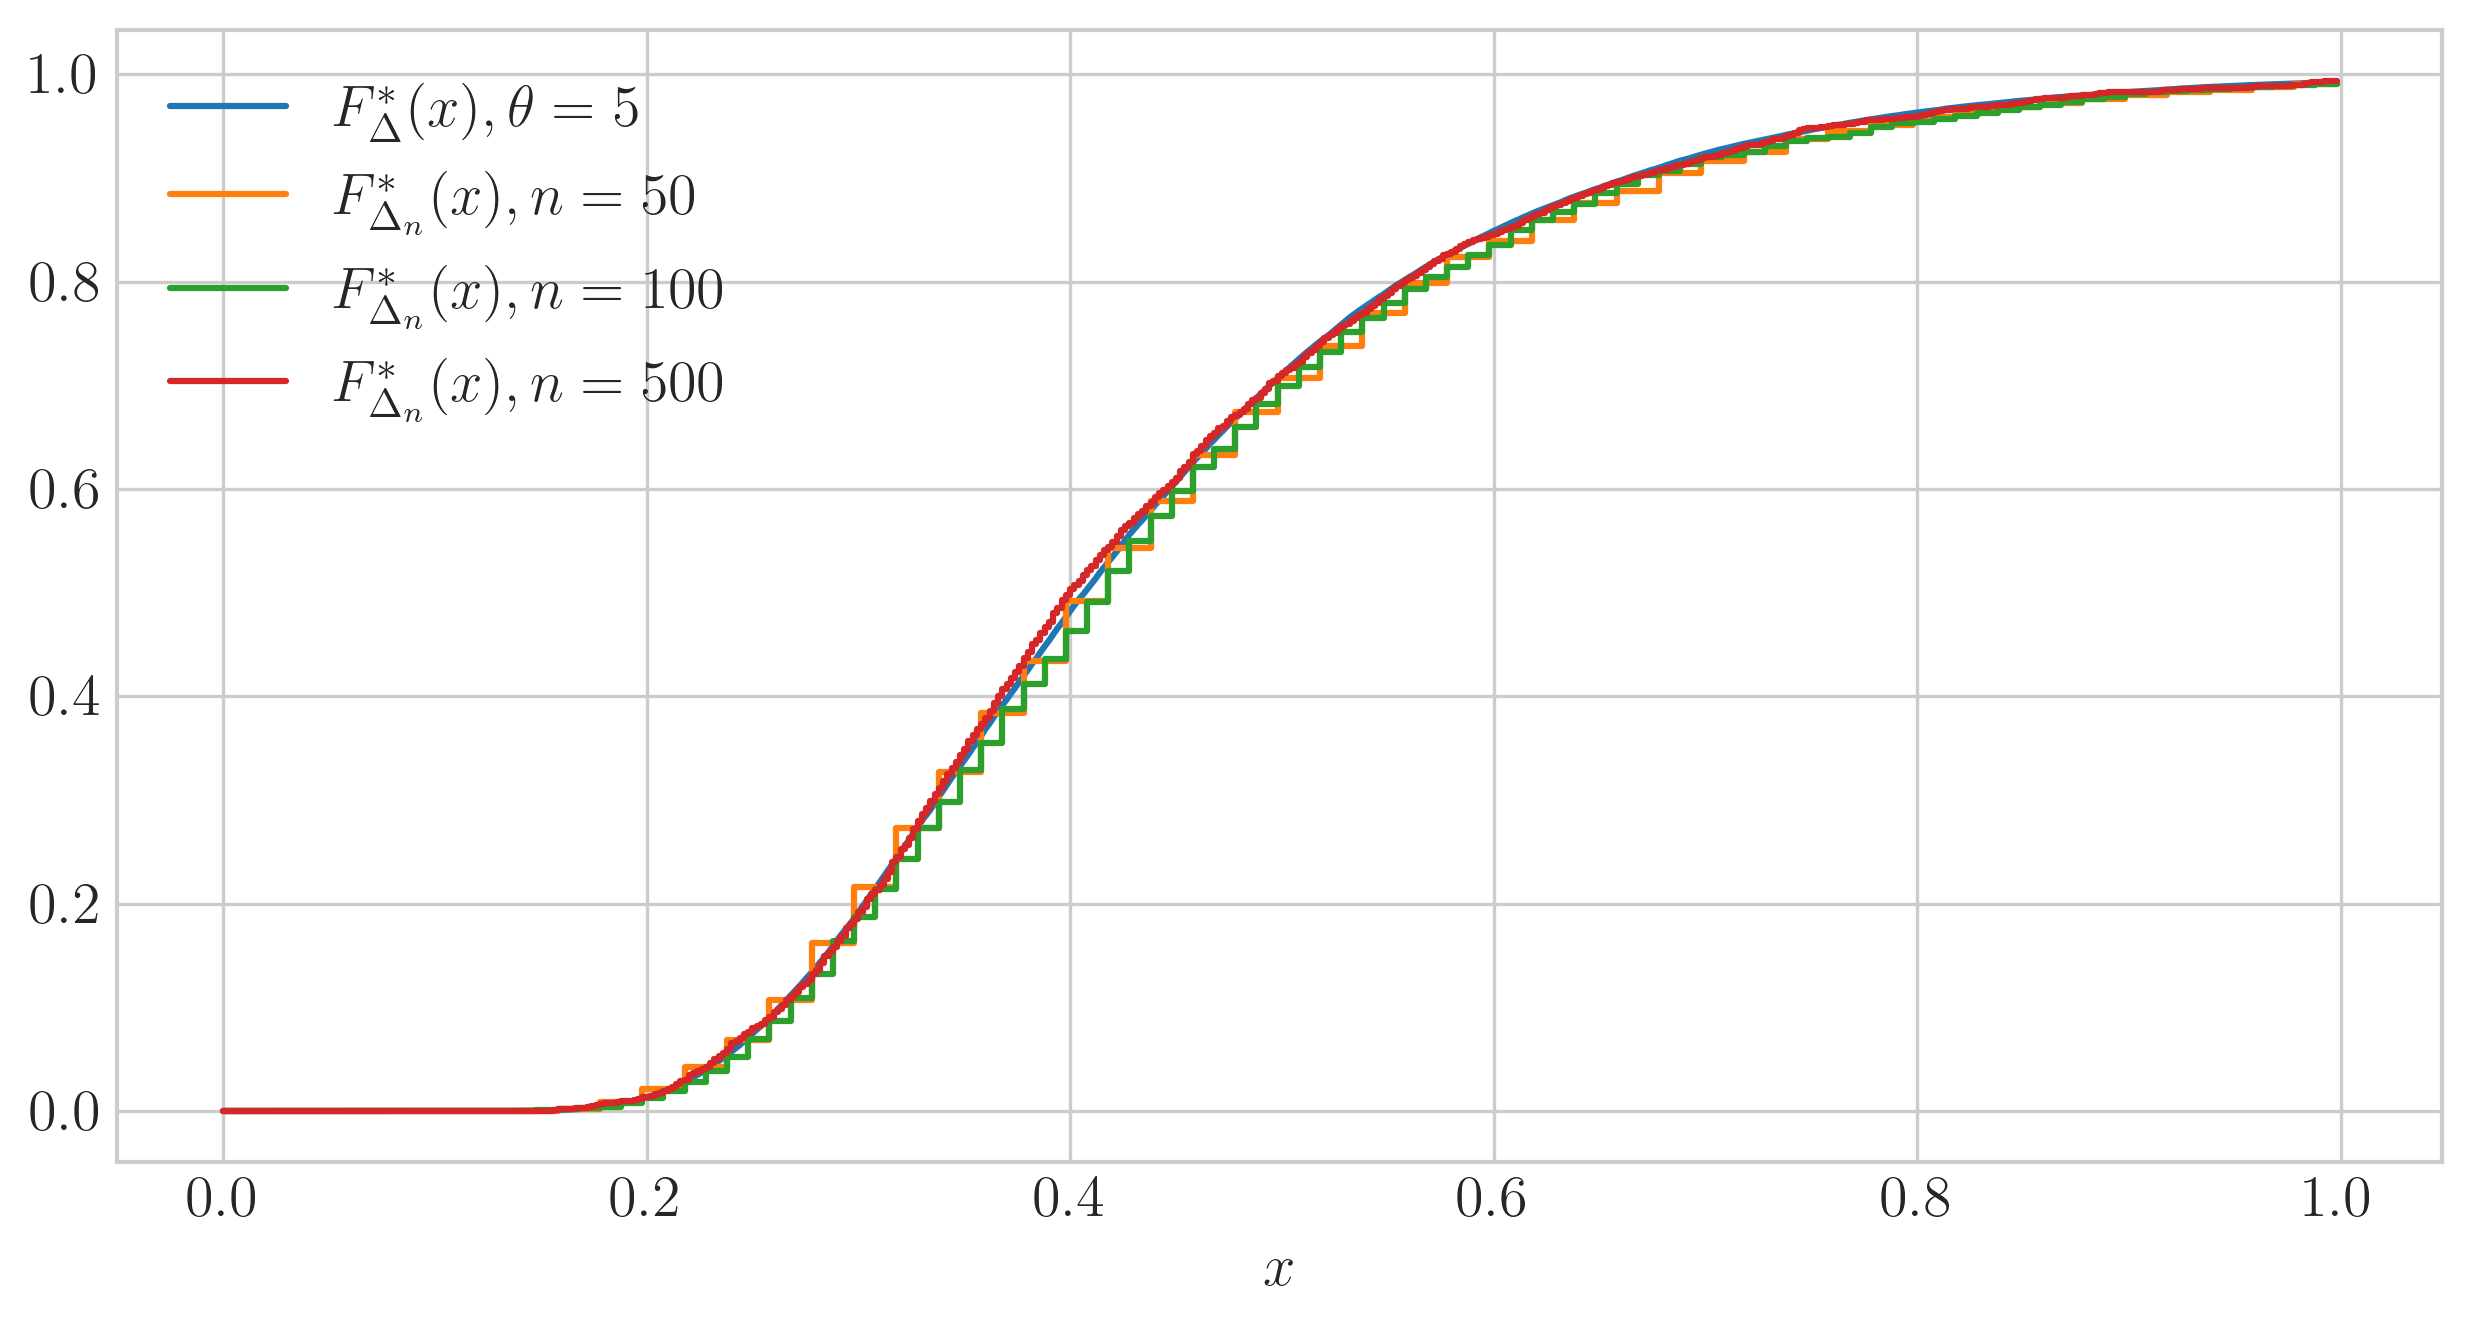
\includegraphics[scale=0.55]{plots/fp_spacing_max_theta_5.png}

            Plots of CDFs of $\Delta$ and $\frac{\Delta_n}{n}$ modelled with CRP for $\theta = 5$.
        \end{center}
    \end{frame}
    \begin{frame}
        \frametitle{Perspectives}
        \begin{enumerate}
            \item \emph{Related results for short cycles}. As it was already mentioned,
            $\cycle_j(\sigma_n)\overset{d}{\longrightarrow} X_j \sim \Poiss{\theta / j}, \; j \in \N$.
            It is reasonable to expect $vd$-convergence of point processes associated with cycles of fixed length $j$
            to a $\theta / j$-rate homogeneous Poisson point process on some appropriate space.
            \item \emph{Functional limit theorems}. As an example, let $X_n(t) = P_{\ceil{n t}}([0, 1])$, $t \in [0, 1]$. 
            It is already known that their one-dimensional distributions weakly converge to
            $\Poiss{\theta}$ as $n \to \infty$. What can be said
            about finite-dimensional convergence? About convergence in $\mathcal{D}_{[0, 1]}$?
            % Chinese restaurant process can be used here, since this coupling
            % allows to generate a sequence $\left(\sigma_i, i\geq 1\right)$ of
            % $\sigma_i \sim \ESF{i, \theta}$ on a common probability space.
            In order for all these questions to make sense, we need to couple 
            all the permutations on a common probability space. 
            As it was mentioned, it can be done by means of the Chinese restaurant process.
        \end{enumerate}
    \end{frame}
    \begin{frame}[allowframebreaks]
        \fontsize{10pt}{12pt}\selectfont
        \nocite{Ewens1972}
        \nocite{ATB1992}
        \nocite{Crane2016}
        \nocite{Kallenberg2017}
        % \nocite{Resnick2007}
        \nocite{Resnick2008}
        % \nocite{LastPenrose2017}
        \nocite{Holst1980}
        \nocite{Renyi1953}
        \nocite{LogStructures}
        \frametitle{References}
        \bibliographystyle{plainyr}
        \bibliography{books.bib}
    \end{frame}
    \begin{frame}
        \begin{minipage}{0.5\textwidth}
            
\includegraphics[width=\linewidth]{plots/cat.png}
        \end{minipage}
        \begin{minipage}{0.4\textwidth}\raggedleft
            \emph{And special thanks to \\ the Armed Forces of Ukraine \\
            for making this presentation possible.}
        \end{minipage}
    \end{frame}
\end{document}